\documentclass[10pt,titlepage,hidelinks]{scrartcl}

\usepackage[default,book,lining,semibold]{FiraSans}
\usepackage{polyglossia}
\usepackage{ragged2e}
\usepackage{calc}
\usepackage{setspace}
\usepackage{graphicx}
\usepackage{hyperref}

\setstretch{1.04}
\setlength{\RaggedRightParindent}{\parindent}
\RaggedRight
\setmainlanguage{finnish}
\addtokomafont{caption}{\itshape}
\newcommand{\scheduler}{\textsc{scheduler}}
\urlstyle{same}

\begin{document}
\title{scheduler}
\author{Janne Suomalainen}
\maketitle

\tableofcontents\clearpage

\section{Johdanto}

\href{https://onlinescheduler.herokuapp.com/}{\scheduler{}} on pieni www-alustainen tietokantajärjestelmä yrityksen työvuorolistojen laatimiseen, jakamiseen ja säilömiseen; ohjelmalla pystyy suunnitella ja tarkastella työvuoroja. Excel-pohjaiset työvuorolistat ovat -- vaikka nerokkaita -- talukkolaskentaan tottumalle epäintuitiivisia käyttää, niiden jakaminen työntekijöille on varsin rajoittunutta ja niiden päivittäminen on työlästä. \scheduler{}-ohjelman tavoitteena on tarjota varteenotettava ratkaisu edellä mainittuihin ongelmiin.

\scheduler{} toteutetaan \href{https://www.heroku.com/}{Heroku}-pilvipalveluun. Pääasiallinen ohjelmointikieli on Java~8; ohjelma käyttää \href{http://sparkjava.com/}{Spark}-nimistä web-sovelluskehystä, Javan tärkeimpiä kirjastoja ja \href{http://www.sql2o.org/}{sql2o}-kirjastoa. Tallennustoiminnallisuudesta vastaa \href{https://www.postgresql.org/}{PostgreSQL}-tietokanta.

\section{Yleiskuva järjestelmästä}

Yleiskuva \scheduler{}-järjestelmän toiminnallisuudesta on esitetty kuvassa~\ref{fig:kayttotapaukset}. Kaavion tueksi annetaan lyhyet kuvaukset järjestelmän sidosryhminä toimivista käyttäjäryhmistä ja esitetään muutama käyttötapauksista tarkemmin.

\begin{figure}[tb]
\centering
\makebox[\textwidth][c]{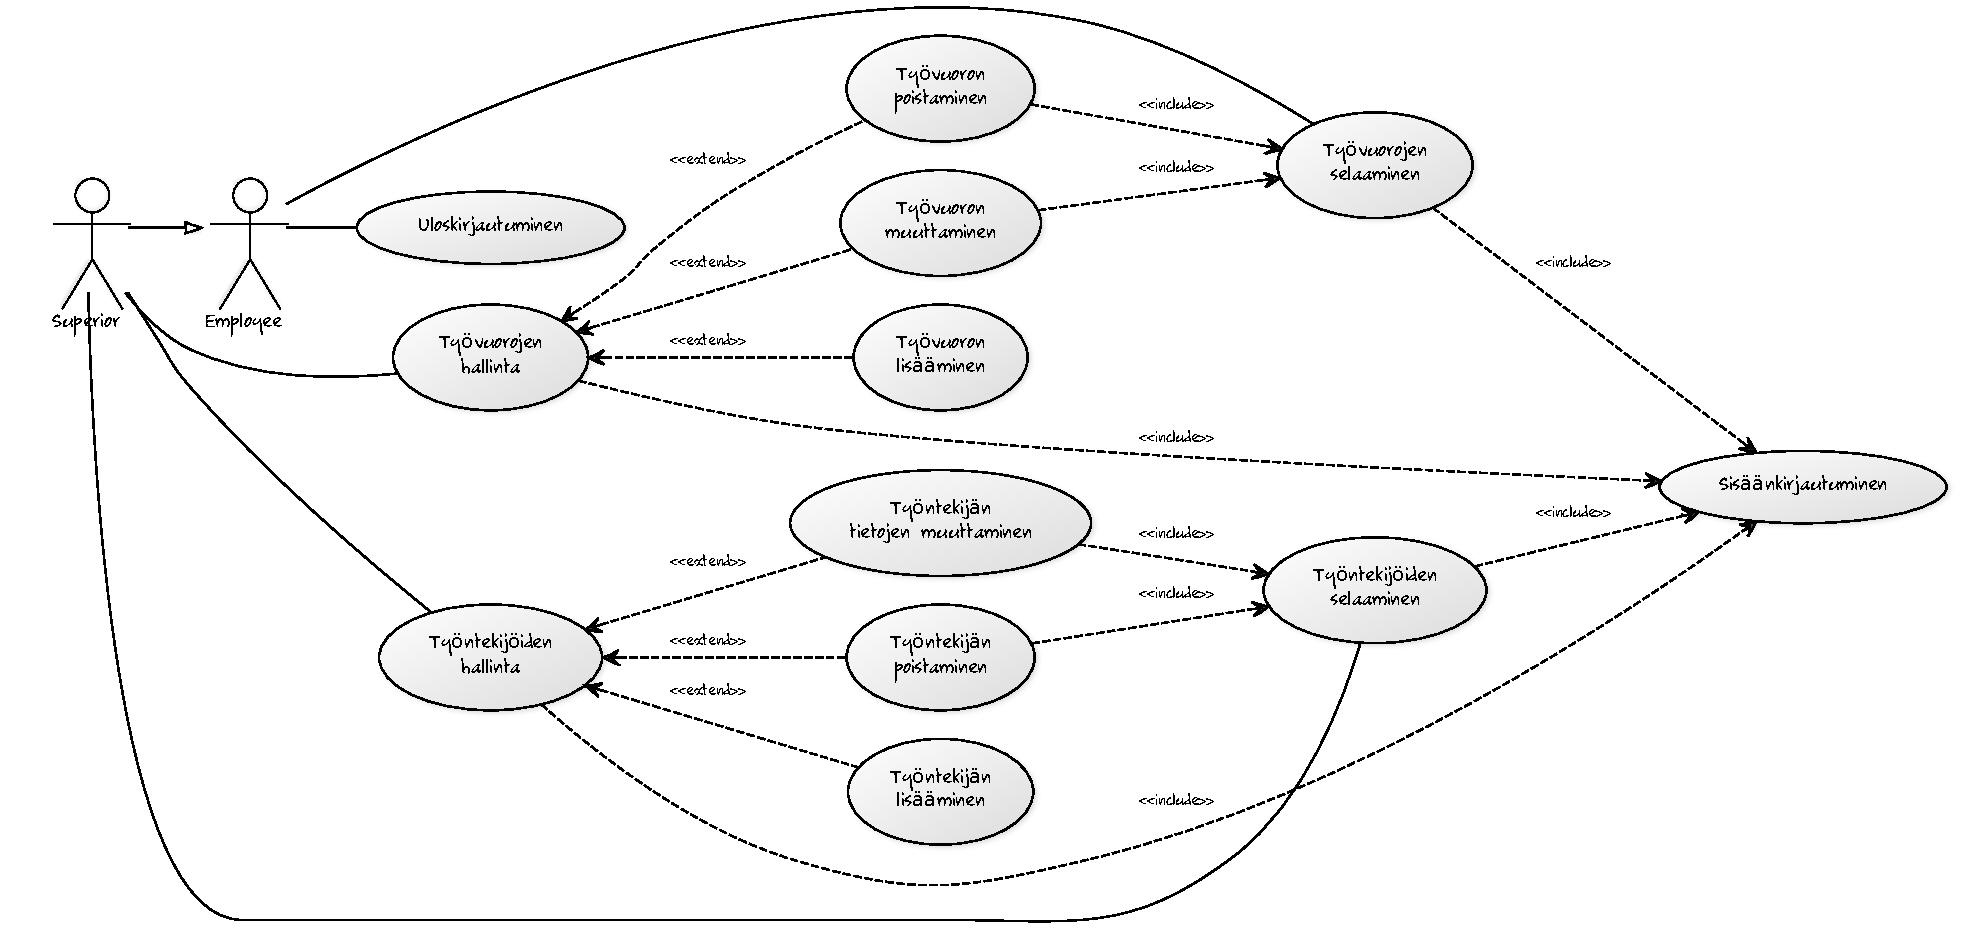
\includegraphics[width=1.5\textwidth]{bfd992e8}}
\caption{Käyttötapauskaavio näyttää järjestelmän sidosryhmät ja miten ne liittyvät järjestelmään.}
\label{fig:kayttotapaukset}
\end{figure}

\begin{description}
\item[Employee] kuvaa tässä yrityksen työntekijää, joka on rekisteröity järjestelmään ja joka ei ole esimiesasemassa.
\item[Superior] on järjestelmään rekisteröity esimiesasemassa toimiva yrityksen työntekijä.
\end{description}

\subsubsection*{Employee selaa työvuoroja}

Käyttötapauksen käyttäjä on työntekijä, jonka tavoitteena on saada tietoa omista työvuoroistaan. Tapauksen esiehtona on, että työntekijä on kirjautunut sisään, jälkiehtona, että työntekijä on saanut tarvitsemansa tiedon työvuoroistaan. Käyttötapaus etenee seuraavasti: \begin{enumerate}
\item Työntekijä aloittaa työvuorojen selaustoiminnon. Hän asettaa haetuille työvuoroille rajoitteita esimerkiksi ajankohdan tai toimipisteen mukaan.
\item Järjestelmä näyttää työntekijälle osoitetut työvuorot ottaen huomioon työntekijän asettamat rajoitteet. \begin{enumerate}
\item Järjestelmä ilmoittaa, mikäli työntekijän asettamat rajoitteet ovat ristiriitaisia.
\item Järjestelmä ilmoittaa, mikäli työntekijän asettamien rajoitteiden mukaisia työvuoroja ei löydy.
\end{enumerate}
\item Työntekijä tutkii työvuoroja.
\end{enumerate}

\subsubsection*{Superior lisää työvuoron}

Käyttötapauksen käyttäjä on esimies, jonka tavoitteena on asettaa työvuoro. Tapauksen esiehtona on, että esimies on kirjautunut sisään, jälkiehtona, että haluttu työvuoro on asetettu. Käyttötapaus etenee seuraavasti: \begin{enumerate}
\item Esimies aloittaa työvuorojen lisäystoiminnon. Hän valitsee asianomaiset työntekijät, toimipisteen ja työvuoron alkamis- ja päättymisajat.
\item Järjestelmä vahvistaa työvuoron lisäyksen. \begin{enumerate}
\item Järjestelmä ilmoittaa, mikäli esimiehen valinnat ovat ristiriitaisia.
\item Järjestelmä ilmoittaa, mikäli työvuoro menee päällekkäin valittujen työntekijöiden aiemmin asetettujen työvuorojen kanssa.
\end{enumerate}
\end{enumerate}

\subsubsection*{Superior muuttaa työvuoroa}

Käyttötapauksen käyttäjä on esimies, jonka tavoitteena on muuttaa jo asetettu työvuoro. Tapauksen esiehtona on, että esimies on kirjautunut sisään ja että työvuoroja on asetettu. Tapauksen jälkiehtona on, että haluttu työvuoro on muutettu. Käyttötapaus etenee seuraavasti: \begin{enumerate}
\item \textbf{Suoritetaan käyttötapaus Työvuorojen selaaminen}.
\item Esimies valitsee muutettavan työvuoron ja käynnistää työvuoron muuttamistoiminnon. Hän valitsee uudet työvuoron alkamis- ja päättymisajat.
\item Järjestelmä vahvistaa työvuoron muuttamisen. \begin{enumerate}
\item Järjestelmä ilmoittaa, mikäli esimiehen valinnat ovat ristiriitaisia.
\item Järjestelmä ilmoittaa, mikäli muutettu työvuoro menee päällekkäin sille asetettujen työntekijöiden muiden työvuorojen kanssa.
\end{enumerate}
\end{enumerate}

\subsubsection*{Superior poistaa työntekijän}

Käyttötapauksen käyttäjä on esimies, jonka tavoitteena on poistaa työntekijä järjestelmästä. Tapauksen esiehtona on, että esimies on kirjautunut sisään, jälkiehtona, että poistettua tyntekijää ei enää löydy järjestelmästä. Käyttötapaus etenee seuraavasti: \begin{enumerate}
\item \textbf{Suoritetaan käyttötapaus Työntekijöiden selaaminen}.
\item Esimies valitsee poistettavan työntekijän ja aloittaa työntekijän poistamistoiminnon.
\item Järjestelmä vahvistaa työntekijän poistamisen.
\end{enumerate}

\section{Järjestelmän tietosisältö}

Järjestelmän tietosisältö kuvataan käsitekaavion (Kuva~\ref{fig:kasitekaavio}) avulla.

\begin{figure}[tb]
\centering
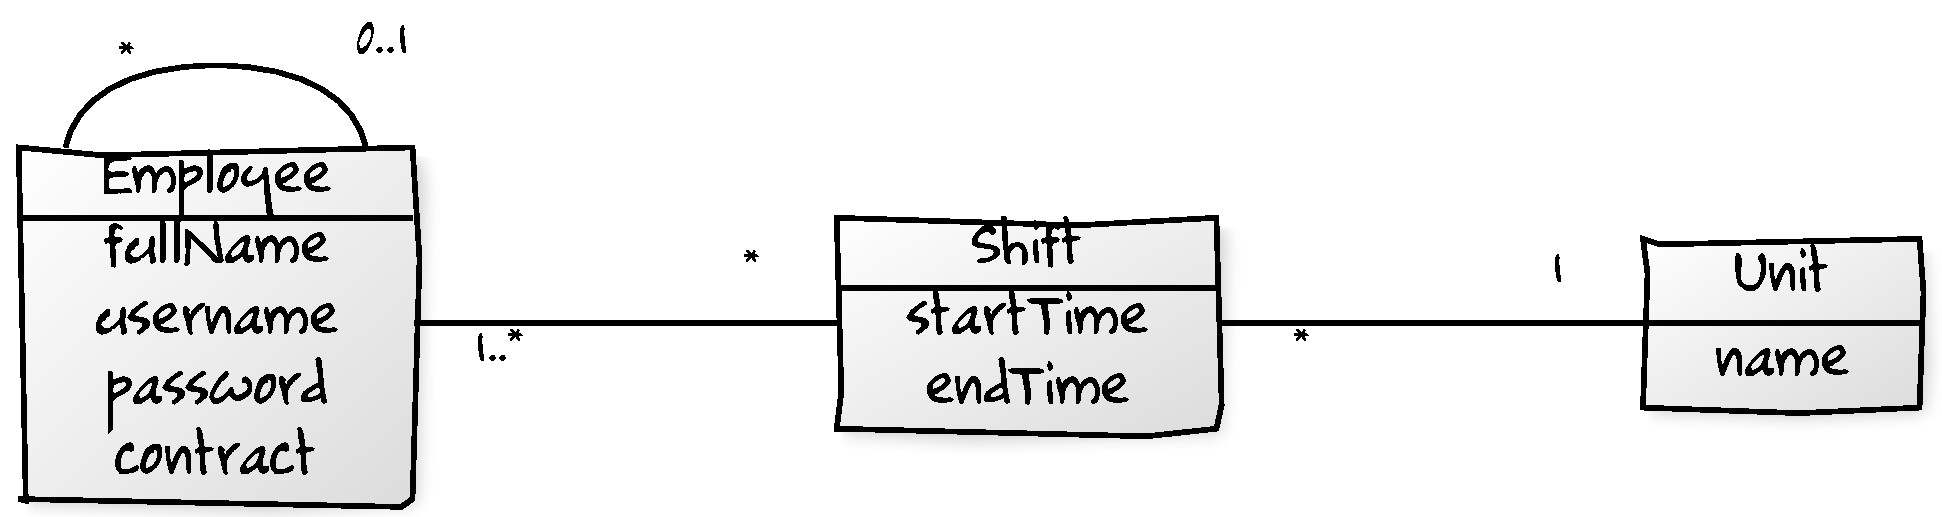
\includegraphics[width=.5\textwidth]{e85adf45}
\caption{Käsitekaavio on järjestelmään säilöttävälle tiedolle käsitetason malli, jonka perusteella johdetaan toteutustason relaatiotietokantakaavio.}
\label{fig:kasitekaavio}
\end{figure}

\section{Relaatiotietokantakaavio}

Alustava \scheduler{}-järjestelmän tietokantakaavio on esitetty kuvassa~\ref{fig:tietokantakaavio}.

\begin{figure}[tb]
\centering
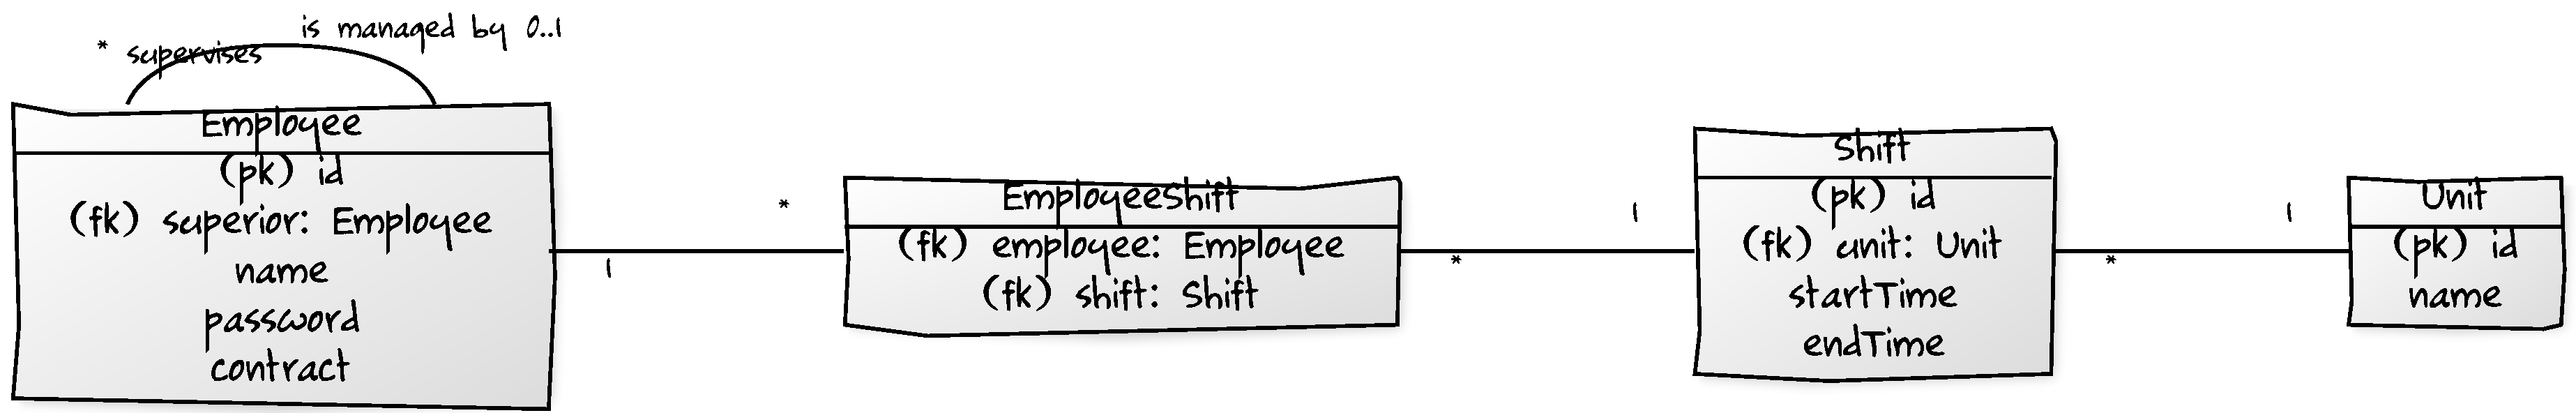
\includegraphics[width=\textwidth]{af410d18}
\caption{Relaatiotietokantakaaviossa tiedon säilömiseen käytettävän tietokannan rakenne esitetään kaaviokuvana.}
\label{fig:tietokantakaavio}
\end{figure}

\section{Järjestelmän yleisrakenne}
\section{Käyttöliittymä ja järjestelmän komponentit}
\section{Asennustiedot}
\section{Käynnistys- tai käyttöohje}
\section{Testaus, tunnetut bugit ja puutteet sekä jatkokehitysideat}
\section{Omat kokemukset}
\end{document}